% Hlavicka pro protokoly z fyzikalniho praktika.
% Verze pro: LaTeX
% Verze hlavicky: 22. 2. 2007
% Autor: Ustav fyziky kondenzovanych latek
% Ke stazeni: www.physics.muni.cz/ufkl/Vyuka/
% Licence: volne k pouziti, nejlepe k vcasnemu odevzdani protokolu z Vaseho mereni.


\documentclass[czech,11pt,a4paper]{article}
\usepackage[T1]{fontenc}
\usepackage{graphicx, animate}
\usepackage{mathtools}
\usepackage{amssymb}
\usepackage{amsthm}
\usepackage{thmtools}
\usepackage{xcolor}
\usepackage{nameref}
\usepackage{babel}
\usepackage{hyperref}
\usepackage{multicol}
\usepackage[export]{adjustbox}
\usepackage{subcaption}
\usepackage{caption}
\usepackage{multirow}
\usepackage{float}
\usepackage{placeins}

\graphicspath{ {./images/} }
\usepackage[backend=biber,style=numeric]{biblatex}       % [1], [2], ...




\addbibresource{ref.bib}


%%% Nemente:
\usepackage[margin=2cm]{geometry}
\newtoks\jmenopraktika \newtoks\jmeno \newtoks\datum
\newtoks\obor \newtoks\skupina \newtoks\rocnik \newtoks\semestr
\newtoks\cisloulohy \newtoks\jmenoulohy

%%% Nemente - konec.


%%%%%%%%%%% Doplnte pozadovane polozky:

\jmenopraktika={Fyzikální praktikum 3}  % nahradte jmenem vaseho predmetu
\jmeno={Teodor Duraković}            % nahradte jmenem mericiho
\datum={22.~dubna 2025}        % nahradte datem mereni ulohy
\obor={F}                     % nahradte zkratkou vami studovaneho oboru
\skupina={Út 14:00}            % nahradte dobou vyuky vasi seminarni skupiny
\rocnik={II}                  % nahradte rocnikem, ve kterem studujete
\semestr={IV}                 % nahradte semestrem, ve kterem studujete

\cisloulohy={11}           % nahradte cislem merene ulohy
\jmenoulohy={Operační zesilovač}           % nahradte vlhkosti vzduchu pri mereni (v %)

%%%%%%%%%%% Konec pozadovanych polozek.


%%%%%%%%%%% Uzitecne balicky:

%%%%%% Zamezeni parchantu:
\widowpenalty 10000 \clubpenalty 10000 \displaywidowpenalty 10000
%%%%%% Parametry pro moznost vsazeni vetsiho poctu obrazku na stranku
\setcounter{topnumber}{3}	  % max. pocet floatu nahore (specifikace t)
\setcounter{bottomnumber}{3}	  % max. pocet floatu dole (specifikace b)
\setcounter{totalnumber}{6}	  % max. pocet floatu na strance celkem
\renewcommand\topfraction{0.9}	  % max podil stranky pro floaty nahore
\renewcommand\bottomfraction{0.9} % max podil stranky pro floaty dole
\renewcommand\textfraction{0.1}	  % min podil stranky, ktery musi obsahovat text
\intextsep=8mm \textfloatsep=8mm  %\intextsep pro ulozeni [h] floatu a \textfloatsep pro [b] or [t]

% Tecky za cisly sekci:
\renewcommand{\thesection}{\arabic{section}.}
\renewcommand{\thesubsection}{\thesection\arabic{subsection}.}
\renewcommand{\thesubsubsection}{\thesubsection\arabic{subsubsection}.}
% Jednopismenna mezera mezi cislem a nazvem kapitoly:
\makeatletter \def\@seccntformat#1{\csname the#1\endcsname\hspace{1ex}} \makeatother


%%%%%%%%%%%%%%%%%%%%%%%%%%%%%%%%%%%%%%%%%%%%%%%%%%%%%%%%%%%%%%%%%%%%%%%%%%%%%%%
%%%%%%%%%%%%%%%%%%%%%%%%%%%%%%%%%%%%%%%%%%%%%%%%%%%%%%%%%%%%%%%%%%%%%%%%%%%%%%%
% Zacatek dokumentu
%%%%%%%%%%%%%%%%%%%%%%%%%%%%%%%%%%%%%%%%%%%%%%%%%%%%%%%%%%%%%%%%%%%%%%%%%%%%%%%
%%%%%%%%%%%%%%%%%%%%%%%%%%%%%%%%%%%%%%%%%%%%%%%%%%%%%%%%%%%%%%%%%%%%%%%%%%%%%%%

\begin{document}
	
	%%%%%%%%%%%%%%%%%%%%%%%%%%%%%%%%%%%%%%%%%%%%%%%%%%%%%%%%%%%%%%%%%%%%%%%%%%%%%%%
	% Nemente:
	%%%%%%%%%%%%%%%%%%%%%%%%%%%%%%%%%%%%%%%%%%%%%%%%%%%%%%%%%%%%%%%%%%%%%%%%%%%%%%%
	\thispagestyle{empty}
	
	{
		\begin{center}
			\sf 
			{\Large Ústav fyziky a technologií plazmatu Přírodovědecké fakulty Masarykovy univerzity} \\
			\bigskip
			{\huge \bfseries FYZIKÁLNÍ PRAKTIKUM} \\
			\bigskip
			{\Large \the\jmenopraktika}
		\end{center}
		
		\bigskip
		
		\sf
		\noindent
		\setlength{\arrayrulewidth}{1pt}
		\begin{tabular*}{\textwidth}{@{\extracolsep{\fill}} l l}
			\large {\bfseries Zpracoval:}  \the\jmeno & \large  {\bfseries Naměřeno:} \the\datum\\[2mm]
			\large  {\bfseries Obor:} \the\obor  \hspace{40mm}  {\bfseries Skupina:} \the\skupina %
			%{\bfseries Ročník:} \the\rocnik \hspace{5mm} {\bfseries Semestr:} \the\semestr  
			&\large {\bfseries Testováno:}\\
			\\
			\hline
		\end{tabular*}
	}
	
	\bigskip
	
	{
		\sf
		\noindent \begin{tabular}{p{3cm} p{0.6\textwidth}}
			\Large  Úloha č. {\bfseries \the\cisloulohy:} \par
			\smallskip
			&\Large \bfseries \the\jmenoulohy  \\[2mm]
		\end{tabular}
	}
	
	\vskip1cm
	
	%%%%%%%%%%%%%%%%%%%%%%%%%%%%%%%%%%%%%%%%%%%%%%%%%%%%%%%%%%%%%%%%%%%%%%%%%%%%%%%
	% konec Nemente.
	%%%%%%%%%%%%%%%%%%%%%%%%%%%%%%%%%%%%%%%%%%%%%%%%%%%%%%%%%%%%%%%%%%%%%%%%%%%%%%%
	
	%%%%%%%%%%%%%%%%%%%%%%%%%%%%%%%%%%%%%%%%%%%%%%%%%%%%%%%%%%%%%%%%%%%%%%%%%%%%%%%
	%%%%%%%%%%%%%%%%%%%%%%%%%%%%%%%%%%%%%%%%%%%%%%%%%%%%%%%%%%%%%%%%%%%%%%%%%%%%%%%
	% Zacatek textu vlastniho protokolu
	%%%%%%%%%%%%%%%%%%%%%%%%%%%%%%%%%%%%%%%%%%%%%%%%%%%%%%%%%%%%%%%%%%%%%%%%%%%%%%%
	%%%%%%%%%%%%%%%%%%%%%%%%%%%%%%%%%%%%%%%%%%%%%%%%%%%%%%%%%%%%%%%%%%%%%%%%%%%%%%%
	
	\begin{multicols}{2}
		\section{Zadání}
		1. Sledujte počet zaznamenaných $\alpha$-částic pro dostatečný počet různých poloh zlaté fólie. Ověřte vztah pro Rutherfordův rozptyl.\\
		2. Ověřte, zda počty zaznamenaných $\alpha$-částic mají Poissonovo rozdělení.
		
		
		\section{Teorie}
		
		Operační zesilovač je základní stavební prvek analogové elektroniky, který se vyskytuje v celé řadě zapojení – od jednoduchých zesilovačů až po aktivní filtry nebo matematické operátory (např. derivátory, integrátory). Základem je diferenční zesilovač, který zesiluje rozdíl napětí mezi dvěma vstupy – invertujícím ($-$) a neinvertujícím ($+$).
		
		Ideální operační zesilovač se vyznačuje následujícími vlastnostmi:
		\begin{itemize}
			\item nekonečné napěťové zesílení $A \to \infty$,
			\item nekonečný vstupní odpor $R_\mathrm{in} \to \infty$ (zanedbatelný vstupní proud),
			\item nulový výstupní odpor $R_\mathrm{out} = 0$,
			\item nekonečná šířka pásma – zesiluje všechny frekvence stejně.
		\end{itemize}
		
		Ve skutečnosti jsou tyto parametry konečné, nicméně dostatečně velké na to, aby v jistých případech umožnily idealizovaný přístup.
		
		\subsection{Invertující zesilovač}
		
		V základním zapojení s invertujícím vstupem (obr. 1) je vstupní napětí přivedeno přes odpor $R_1$ na invertující vstup, zatímco neinvertující vstup je uzemněn. Výstup je připojen zpětnovazebním odporem $R_2$ zpět na invertující vstup. Výstupní napětí je pak dáno vztahem:
		\begin{equation}
			U_\mathrm{O} = -\frac{R_2}{R_1} U_1.
		\end{equation}
		Výstupní napětí je inverzní vůči vstupnímu, což je způsobeno právě zapojením na invertující vstup.
		
		
	\begin{figure}[H]
		\centering
		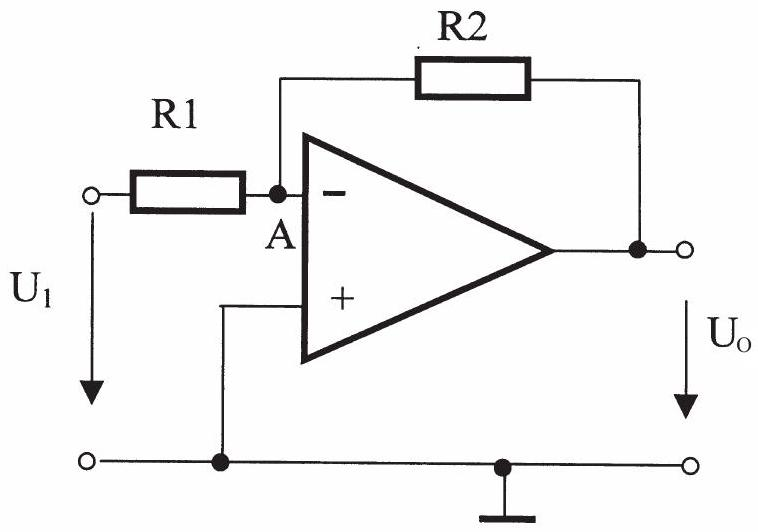
\includegraphics[width=0.8\linewidth]{inv}
		\caption{Zapojení invertujícího zesilovače}
		\label{fig: Zapojení invertujícího zesilovače}
	\end{figure}

		
		\subsection{Neinvertující zesilovač}
		
		U neinvertujícího zesilovače (obr. 2) je vstupní napětí přivedeno na neinvertující vstup. Invertující vstup je připojen ke zpětnovazební děličové síti tvořené rezistory $R_1$ a $R_2$ (viz obr. 6 v zadání). Díky vysokému zesílení a záporné zpětné vazbě platí:
		\begin{equation}
			U_- = U_+ = U_1.
		\end{equation}
		Důsledkem děliče napětí platí:
		\begin{equation}
			U_- = \frac{R_1}{R_1 + R_2} U_\mathrm{O}.
		\end{equation}
		Po dosazení a úpravě dostáváme:
		\begin{equation}
			U_1 = \frac{R_1}{R_1 + R_2} U_\mathrm{O},
		\end{equation}
		\begin{equation}
			U_\mathrm{O} = U_1 \left( 1 + \frac{R_2}{R_1} \right).
		\end{equation}
		
		Zesílení neinvertujícího zapojení tedy musí být vždy větší než jedna.
		\begin{figure}[H]
			\centering
			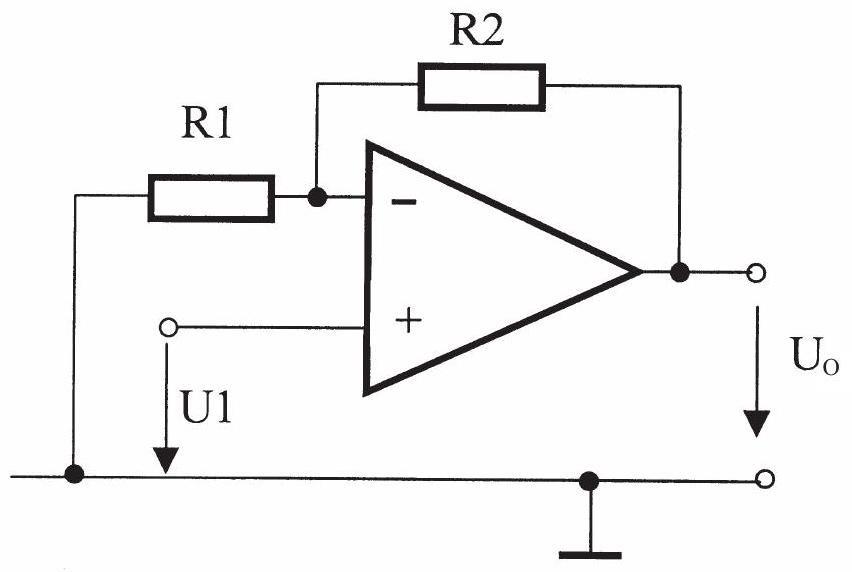
\includegraphics[width=0.8\linewidth]{noninv}
			\caption{Zapojení neinvertujícího zesilovače}
			\label{fig:noninv}
		\end{figure}
		\subsection{Komparátor}
		
		Jedním z nejjednodušších využití operačního zesilovače je tzv. komparátor – zapojení bez zpětné vazby (obr. 3), které srovnává (komparuje) dvě napětí. Výstupní napětí pak nabývá hodnoty blízké napájecímu napětí (kladnému nebo zápornému), v závislosti na tom, které ze vstupních napětí je větší.
		
		\begin{equation}
			U_\mathrm{O} \approx 
			\begin{cases}
				+U_\mathrm{sat}, & \text{pokud } U_+ > U_-, \\
				-U_\mathrm{sat}, & \text{pokud } U_+ < U_-,
			\end{cases}
		\end{equation}
		
		kde $U_\mathrm{sat}$ je mezní (saturační) hodnota výstupního napětí, obvykle blízká napájecímu napětí OZ. Vzhledem k absenci zpětné vazby se operační zesilovač nechová lineárně, ale jako nelineární prvek, který rozhoduje pouze o znaménku rozdílu vstupních napětí.
		
		\begin{figure}[H]
			\centering
			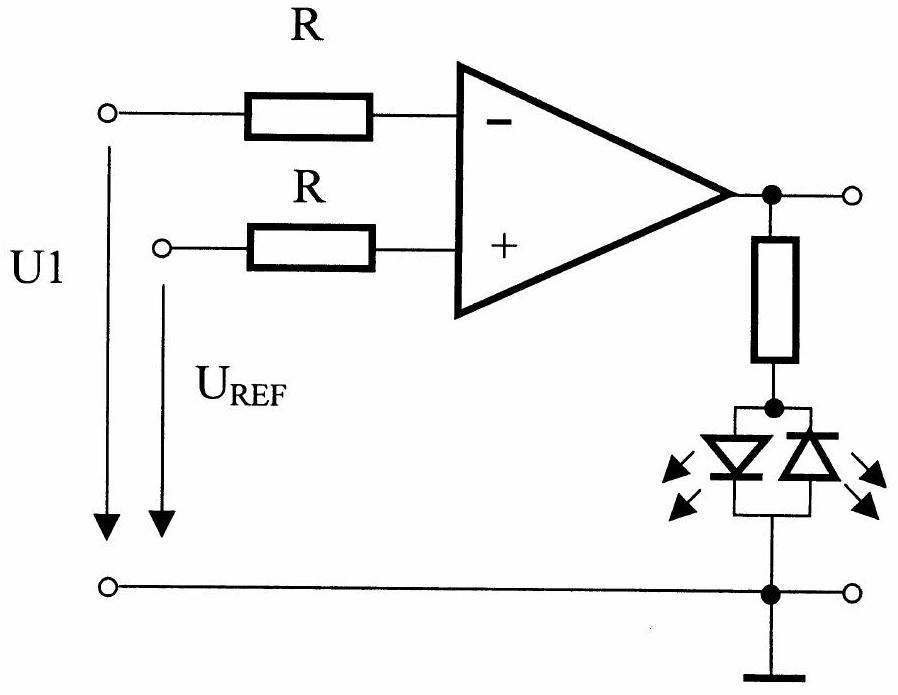
\includegraphics[width=0.8\linewidth]{komp}
			\caption{Zapojení komparátoru}
		\end{figure}
		
		\subsection{Dolnofrekvenční propust}
		
		Přidáním kondenzátoru do zpětnovazební větve invertujícího zesilovače vznikne dolnofrekvenční filtr (obr. 4). Komplexní zesílení tohoto zapojení je dáno vztahem:
		\begin{equation}
			A_u(\omega) = -\frac{R_\mathrm{F}}{R_\mathrm{A}} \cdot \frac{1}{1 + i \omega C_\mathrm{F} R_\mathrm{F}},
		\end{equation}
		kde $C_\mathrm{F}$ je zpětnovazební kondenzátor. Tento filtr propouští signály s nízkou frekvencí a potlačuje vysokofrekvenční složky.
		\begin{figure}[H]
			\centering
			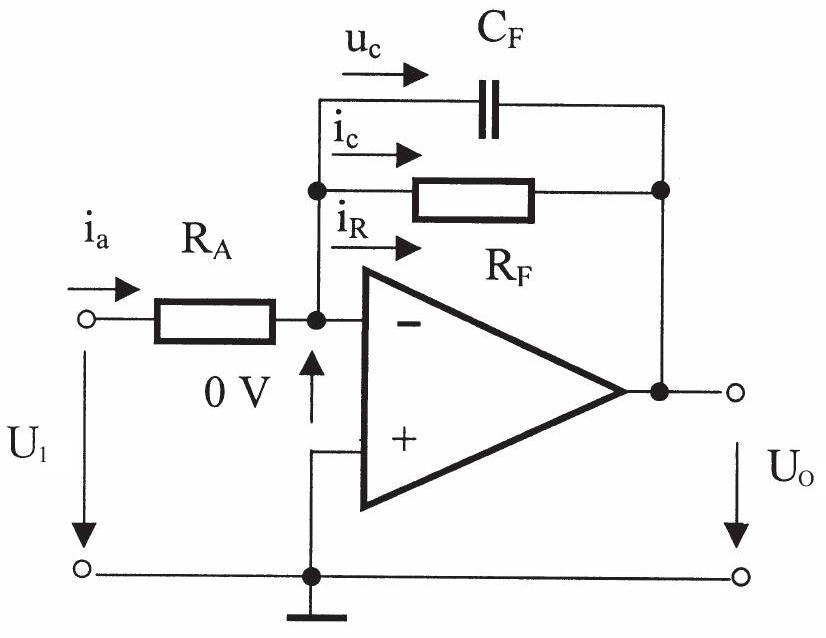
\includegraphics[width=0.8\linewidth]{freq}
			\caption{Zapojení operačního zesilovače pro získání dolnofrekvenční propusti}
		\end{figure}
		\subsection{Rozdílový zesilovač}
		
		Rozdílový zesilovač (obr. 5) zesiluje rozdíl obou vstupních napětí. Formule
		\begin{equation}
			U_\mathrm{O} = 2(U_2 - U_1),
		\end{equation}
		platí při zvolených odporech: $R_1 = R_3 = 10\,\mathrm{k\Omega}$ a $R_2 = R_4 = 20\,\mathrm{k\Omega}$.
		\begin{figure}[H]
			\centering
			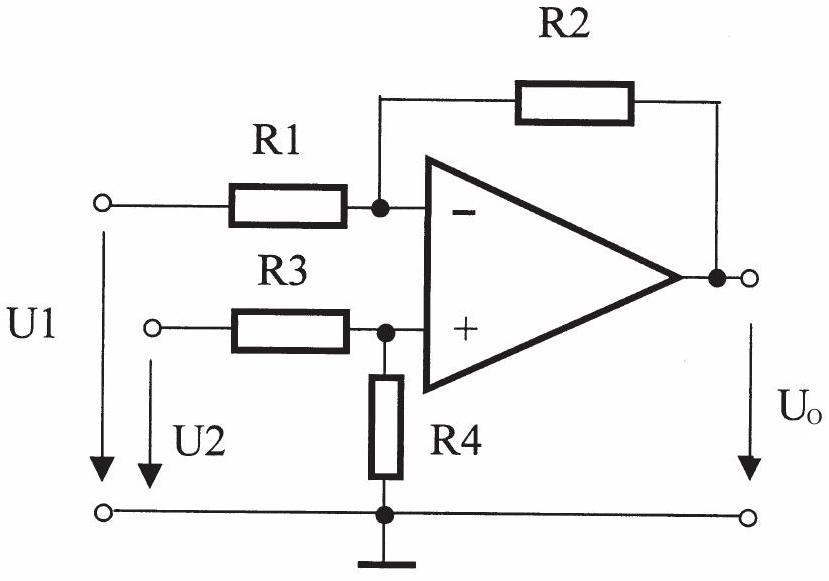
\includegraphics[width=0.8\linewidth]{rozd}
			\caption{Zapojení rozdílového zesilovače}
		\end{figure}
		\subsection{Derivátor}
		
		Pokud je vstupní signál přiveden na kondenzátor a zpětná vazba je tvořena rezistorem, výstupní napětí odpovídá derivaci vstupního signálu:
		\begin{equation}
			U_\mathrm{O}(t) = -RC \frac{\mathrm{d}U_\mathrm{in}(t)}{\mathrm{d}t}.
		\end{equation}
		Zesilovač v tomto zapojení (obr. ) plní funkci derivátoru.
		\begin{figure}[H]
			\centering
			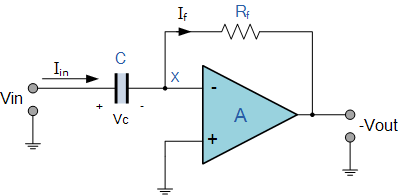
\includegraphics[width=0.8\linewidth]{der}
			\caption{Zapojení derivátoru}
		\end{figure}
		
		
		
		\section{Měření}
		\subsection{Měření se stejnosměrným proudem}
		
		\subsubsection{Invertující zesilovač}
		Zapojujeme odpory $R1 = 10\,\mathrm{k\Omega},\, R2 = 20 \,\mathrm{k\Omega}$, dle formule (1) očekáváme tedy zesílení o velikosti $A = -2$. Kromě experimentálně získaných dat simulujeme i zapojení v programu NI Multisim (obr.7), kde zapojujeme stejný typ operačního zesilovače (TI UA741CP) a očekáváme tedy velmi podobné výsledky. Skutečně pro závislosti vstupního a výstupního napětí získáváme velmi malou odchylku, jak lze pozorovat na obr. 8.
		
		\begin{figure}[H]
			\centering
			
			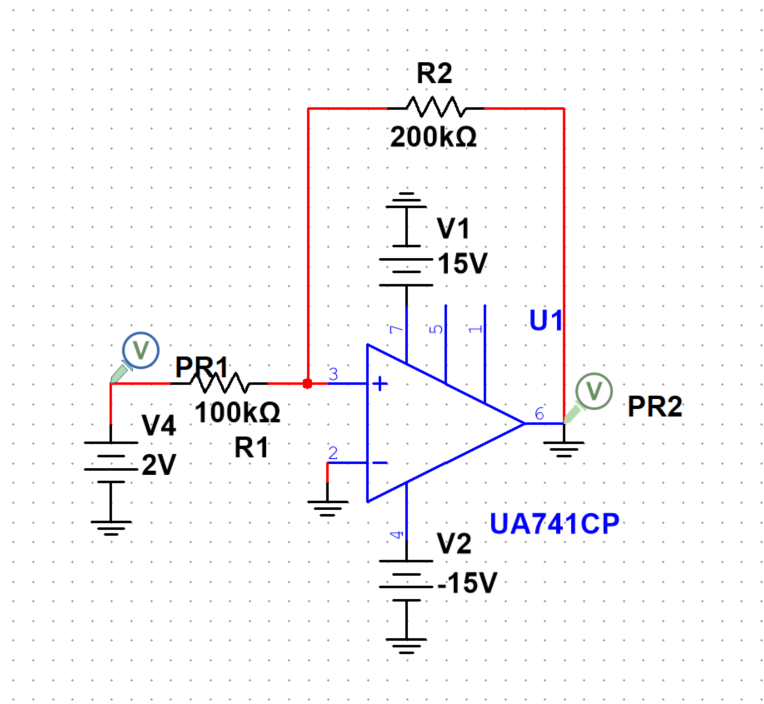
\includegraphics[width=0.8\linewidth]{MSinv}
			\caption{Zapojení pro simulaci v programu Multisim}
			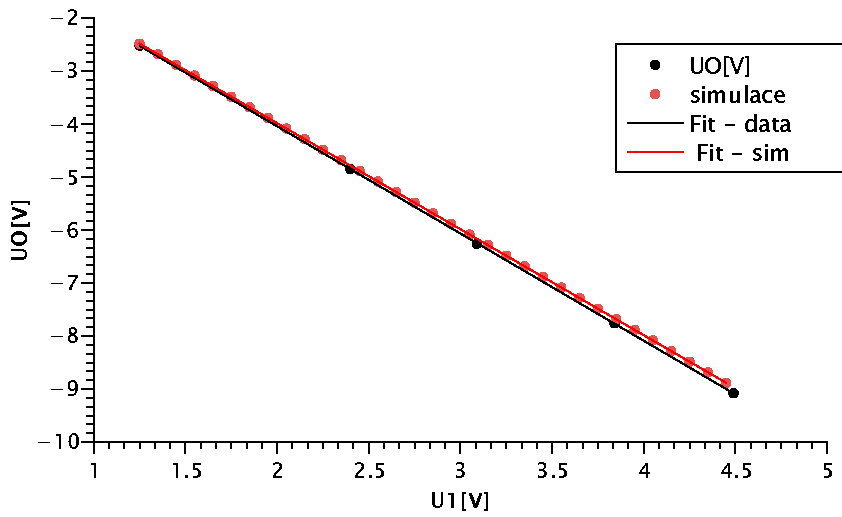
\includegraphics[width=0.8\linewidth]{invz}
			\caption{Experimentální a teoretická závislost vstupního a výstupního napětí}
		\end{figure}
		Pro obě metody lineárním fitem získáváme zesílení:
		\begin{gather}
			A_{exp} =  -2.0221 \pm 0.0012    \\
			A_{sim} =   -1.9950 \pm  0.0003    
		\end{gather}
		Hodnoty se od předpokládané odchylují o méně než procento. U simulované hodnoty lze tuto odchylku vysvětlit ofsetovým napětím (datasheet \cite{TI} udává max. 7.5 mV). Naopak u experimentální hodnoty může být odchylka kromě ofsetového napětí způsobena odchylkou skutečného odporu od udávaného. Toleranci rezistorů jsme nestudovali, nicméně je velmi pravděpodobné, že se jednalo o rezistory s tolerancí 5 nebo 10 procent. V takovém případě je odchylka v očekávaných mezích - stejný výsledek bychom získali i při jednoprocentní toleranci odporu.
		
		\subsubsection{Neinvertující zesilovač}
		Při zapojení podle obr.2 za hodnoty odporů volíme $R1=100 \,\mathrm{k\Omega}, \, R2 = 200 \,\mathrm{k\Omega}$. Dle formule (5) tedy předpokládáme hodnotu zesílení $A=3$. Tento předpoklad je ověřen simulovanými daty (obr. 9) i praktickým měřením - získáváme v podstatě identické hodnoty, což lze pozorovat na obr. 10.
		
		\begin{figure}[H]
			\centering
			
			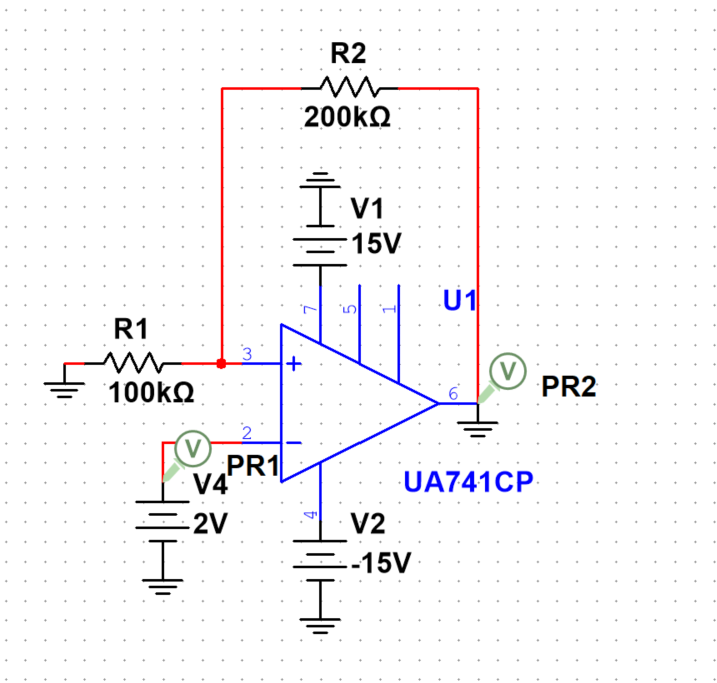
\includegraphics[width=0.8\linewidth]{MSneinv}
			\caption{Zapojení pro simulaci v programu Multisim}
			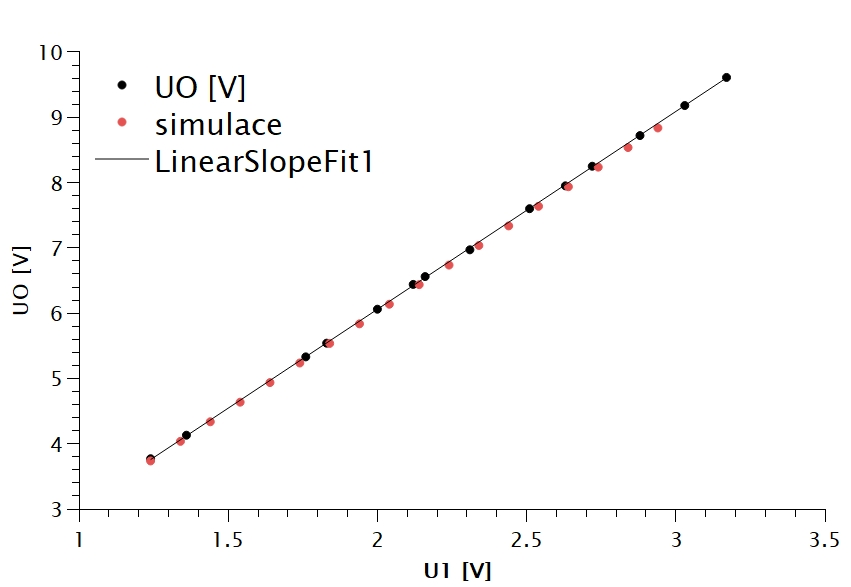
\includegraphics[width=0.8\linewidth]{neinvvys}
			\caption{Experimentální a teoretická závislost vstupního a výstupního napětí}
		\end{figure}
		
		Z lineárního fitu získáváme hodnotu směrnice, a tím i zesílení:
		\begin{equation}
			A =  3.0296 \pm 0.0015
		\end{equation}
		Což se od předpokládaných $A=3$ odchyluje o méně než procento, Odchylku lze znovu vysvětlit vlastnostmi komponent v obvodu.
		\subsubsection{Komparátor}
		V zapojení dle obr. 3 získáváme funkci komparátoru - výstup srovnává invertující a neinvertující vstup. Při větším invertujícím vstupu měříme na výstupu záporné napětí (-11.4 V), při větším neinvertujícím vstupu měříme napětí kladné (12.76 V). Při našem zapojení se v prvním případě rozsvítí červená dioda, v případě druhém dioda zelená - při opačném zapojení komponentu s diodami bychom samozřejmě získali obrácený výsledek.
		\subsubsection{Rozdílový zesilovač}
		Zesilovač zapojujeme dle návodu, předpokládáme tedy chování dle formule (8). Napětí U1 držíme na hodnotě $U1 = 5.06\,\mathrm{V}$ závislost U2/U0 lze sledovat na obr. 11.
		\begin{figure}[H]
			\centering
			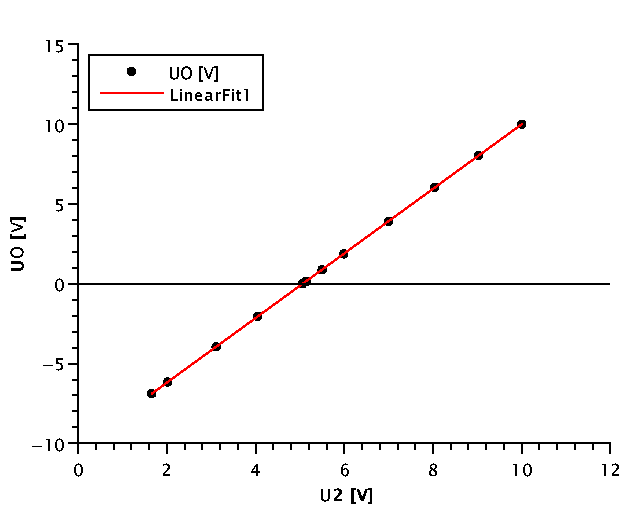
\includegraphics[width=0.8\linewidth]{Graph5}
			\caption{Závislost výstupního napětí na na napětí U2}
		\end{figure}
		Z lineárního fitu lze získat hodnotu U1 a zesílení:
		$U1 = 5.123 \pm 0.002\,\mathrm{V}, A = 2.0242 \pm 0.0008$
		Jelikož používáme stejné rezistory jako v úloze 3.1.1 a získáváme velmi podobné zesílení, je velmi pravděpodobné, že tato odchylka skutečně pramení z tolerancí rezistorů.
		\subsection{Měření se střídavým proudem}
		\subsubsection{Invertující zesilovač}
		Při zapojení zesilovače jako invertujícího generujeme sinusoidální signál na $U_1$ a pozorujeme výstup - $U_O$. Snažíme se určit šířku pásma - hraničním výstupem je výstup s poklesem o 3dB oproti zesílení nízkofrekvenčních signálů. Pro zesílení toto odpovídá poklesu $A_{u,max}\sqrt{2}$ Odpory volíme tak, aby $A=-2$ (tj $10,20 \,\mathrm{k\Omega}$), amplitudu signálu nastavujeme na konstantní $U_1 = 2\,\mathrm{V}$. Pro prahové zesílení tedy platí $A_{min} = 2/\sqrt{2} = \sqrt{2}$, pro amplitudu výstupu $U_{0, min} = 2\sqrt{2}\approx 2.828$. Pro určení přibližné mezní frekvence lze využít závislost maximálního výstupního napětí na frekvenci z datasheetu (obr. 12) - pozorujeme, že tato hodnota odpovídá frekvenci cca. 52 kHz.
		\begin{figure}[H]
			\centering
			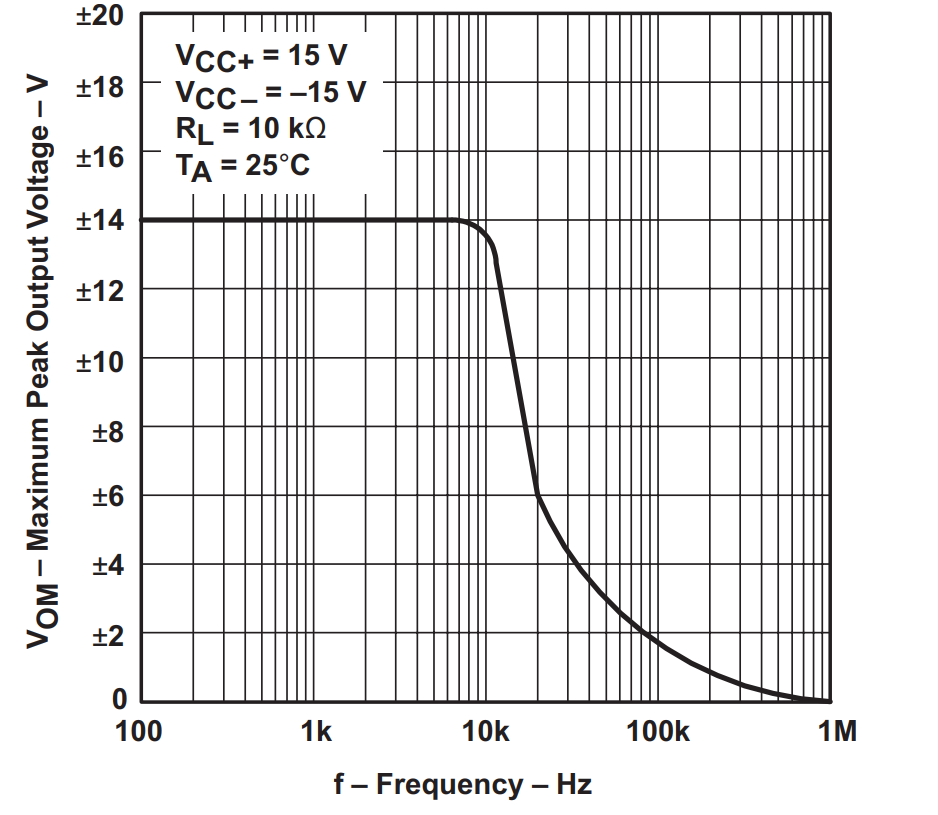
\includegraphics[width=0.8\linewidth]{MSinv1}
			\caption{Závislost maximálního výstupního napětí na frekvenci podle datasheetu}
			\label{fig:msinv1}
		\end{figure}
		Jako mez získáváme hodnotu \\
		$f = 40\,792 \pm 7191 \,\mathrm{Hz}$ (obr.13)
		
		\begin{figure}[H]
			\centering
			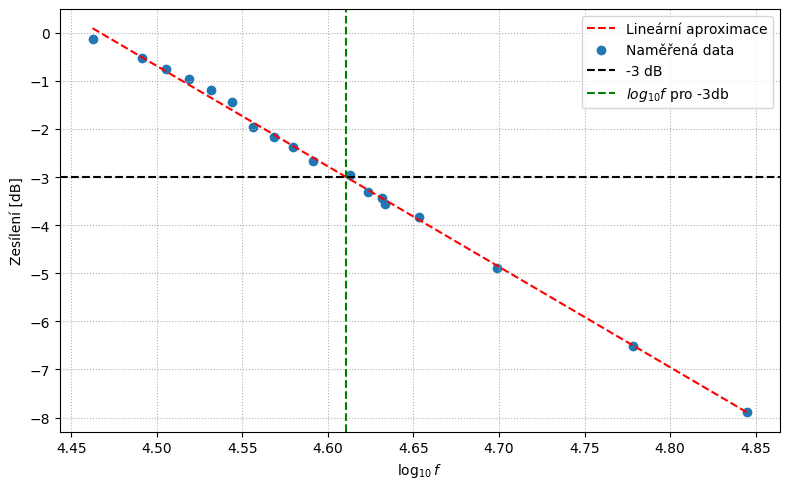
\includegraphics[width=0.8\linewidth]{3dn}
			\caption{Závislost zesílení na $log_{10} f$}
			\label{fig:msinv1}
		\end{figure}
		\subsubsection{Dolnofrekvenční propust}
		Po zapojení při hodnotě kondenzátoru $C = 10 \,\mathrm{nF}$ a hodnotě odporu $RA =20 \,\mathrm{k\Omega}$ očekáváme pětinásobné zesílení, proto je hraniční napětí pro určení šířky pásma $UO = 7.3645 \,\mathrm{V}$.  Přesně tuto hodnotu získáváme pro frekvenci $f = 163 \,\mathrm{Hz}$.
		Vývoj napětí a zesílení lze sledovat na obr. 14.
		\begin{figure}[H]
			\centering
			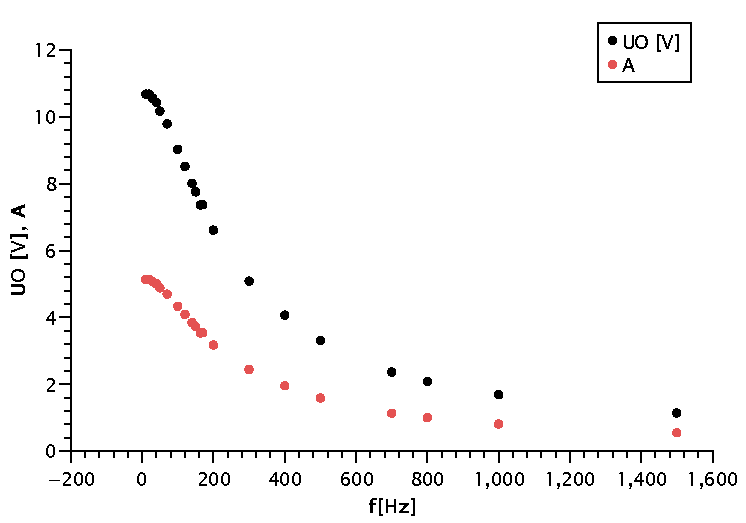
\includegraphics[width=0.8\linewidth]{Graph6}
			\caption{Závislost zesílení a výstupního napětí na frekvenci}
		\end{figure}
		Zároveň dle očekávání při vyšších frekvencích pozorujeme znatelný fázový rozdíl mezi vstupním a výstupním signálem - pro vyšší frekvence se totiž začínají projevovat vlastnosti kondenzátoru. Při hraničních frekvenci je tento fázový rozdíl zhruba desetistupňový. 
		\subsubsection{Derivátor}
		Obvod znovu zapojujeme dle instrukcí, generujeme signál o amplitudě $U_{max} = 1\,\mathrm{V}$. Kromě samotné inverze (již musíme očekávat kvůli napětí na invertující větvi) pozorujeme aditivní fázový posuv $\varphi = 90^\circ$ - derivátor totiž ze vstupní funkce - sinu tvoří její derivaci - kosinus. Celkově tedy sledujeme fázový rozdíl $\varphi = -90^\circ$
		
	
		
		\section{Závěr}
		Podařilo se nám využít všech uvedených funkcí operačního zesilovače, při všech jsme pozorovali očekávané chování, odchylky od teorie se nám též podařilo vysvětlit.
	\end{multicols}
\printbibliography
			
		
		
		% Nakonec nezapomeňte projet text programem vlna nebo vlnka, např.
		% 	vlna -m -l -n mojeuloha.tex
		% nebo zkontrolovat a opravit jednopísmenné předložky na koncích řádků ručně.

\end{document}
